\chapter{Experiment: hardware system}
In this chapter, we discuss experiments conducted on the hardware system. The content is organized into four sections. The first section provides an overview of the hardware setup for the double pendulum system. The second section delves into the system identification of the hardware. The third section details our approach to addressing the sim-to-real gap challenge. The final section presents the successful outcomes of our hardware experiments.

\section{Hardware setup}
Mechanically, the double pendulum system is a straightforward 2-R linkage. The first revolute joint attaches to the base, while the second one connects the two links. Quasi-direct drive motors are mounted on each joint to provide torque, and a counterweight is positioned at the end of the second link.

Our mechanical design for the double pendulum underwent two iterations. In the initial design, the base consisted of a bent aluminum plate, and the links featured a sandwich structure with aluminum on the outside and engineering plastic on the inside. These links were of homogeneous size, meaning that the cross-sectional areas at the link intersections were consistent. We abandoned this design due to rotational imbalances. Specifically, the rotation plane of the links wasn't consistently perpendicular to the motor axes, leading to vibrations and accelerated wear during regular use. In extreme cases, when the links rotated at high angular velocities, this imbalance was exacerbated. This not only resulted in the links bending but also led to catastrophic system failures. Such failures presented significant safety risks to personnel.

In the second iteration, we addressed the issues encountered in the previous design, leading to two major modifications. First, we replaced the aluminum-plastic combination with a carbon fiber-foam blend. While the incorporation of carbon fiber marginally increased the cost, it significantly boosted the yield strength. Second, we introduced triangular-shaped links with central cutouts. This design, while lightweight, also substantially enhanced the yield strength due to the changed intersections. Overall, this iteration resulted in a mechanical structure that is considerably more reliable than the first.
\begin{figure}[htbp]
\begin{minipage}[b]{0.45\linewidth}
\centering
\fbox{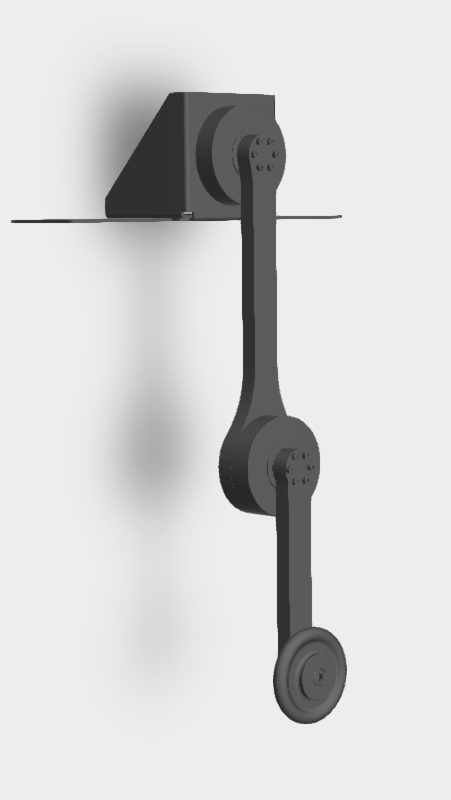
\includegraphics[width=0.75\linewidth]{figures/double_pendulum_CAD.png}}
\end{minipage}
% Example to add your own logos for Acknowledgment
%\hfill
\begin{minipage}[b]{0.45\linewidth}
\centering
\includegraphics[width=1.0\linewidth]{figures/double_pendulum_real_system.png}
\end{minipage}
\caption{Double pendulum setup in CAD (version 1) and in real world (version 2)}
\end{figure}

For the quasi-direct drive motors, we selected the AK80-6 V100 motors from the company CubeMars. This motor's design facilitates easy mounting from both the front and rear ends. As depicted in Figure5.2(b), the motor's maximum torque during continuous operation is 6 Nm, which aligns well with our torque limit of 5 Nm. Additionally, the motor is designed for compatibility with both serial bus and CAN bus, simplifying the development process.


\begin{figure}[htbp]
  \centering
  \begin{subfigure}[b]{0.45\textwidth}
    \centering
    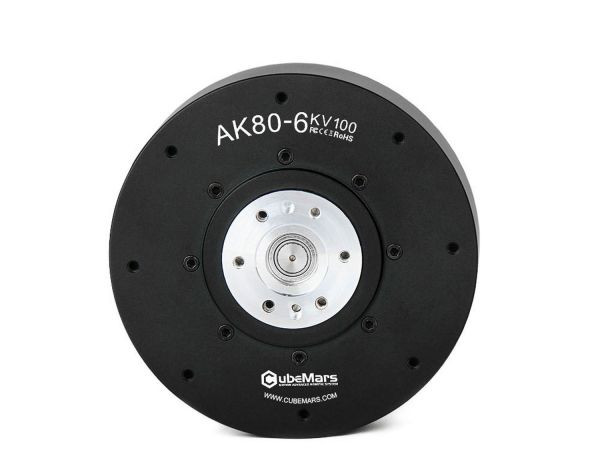
\includegraphics[width=\textwidth]{figures/hardware_setup/motor.jpg}
    \caption{AK80-6 V100 motor}
    \label{fig:subfiga}
  \end{subfigure}
  \hfill
  \begin{subfigure}[b]{0.45\textwidth}
    \centering
    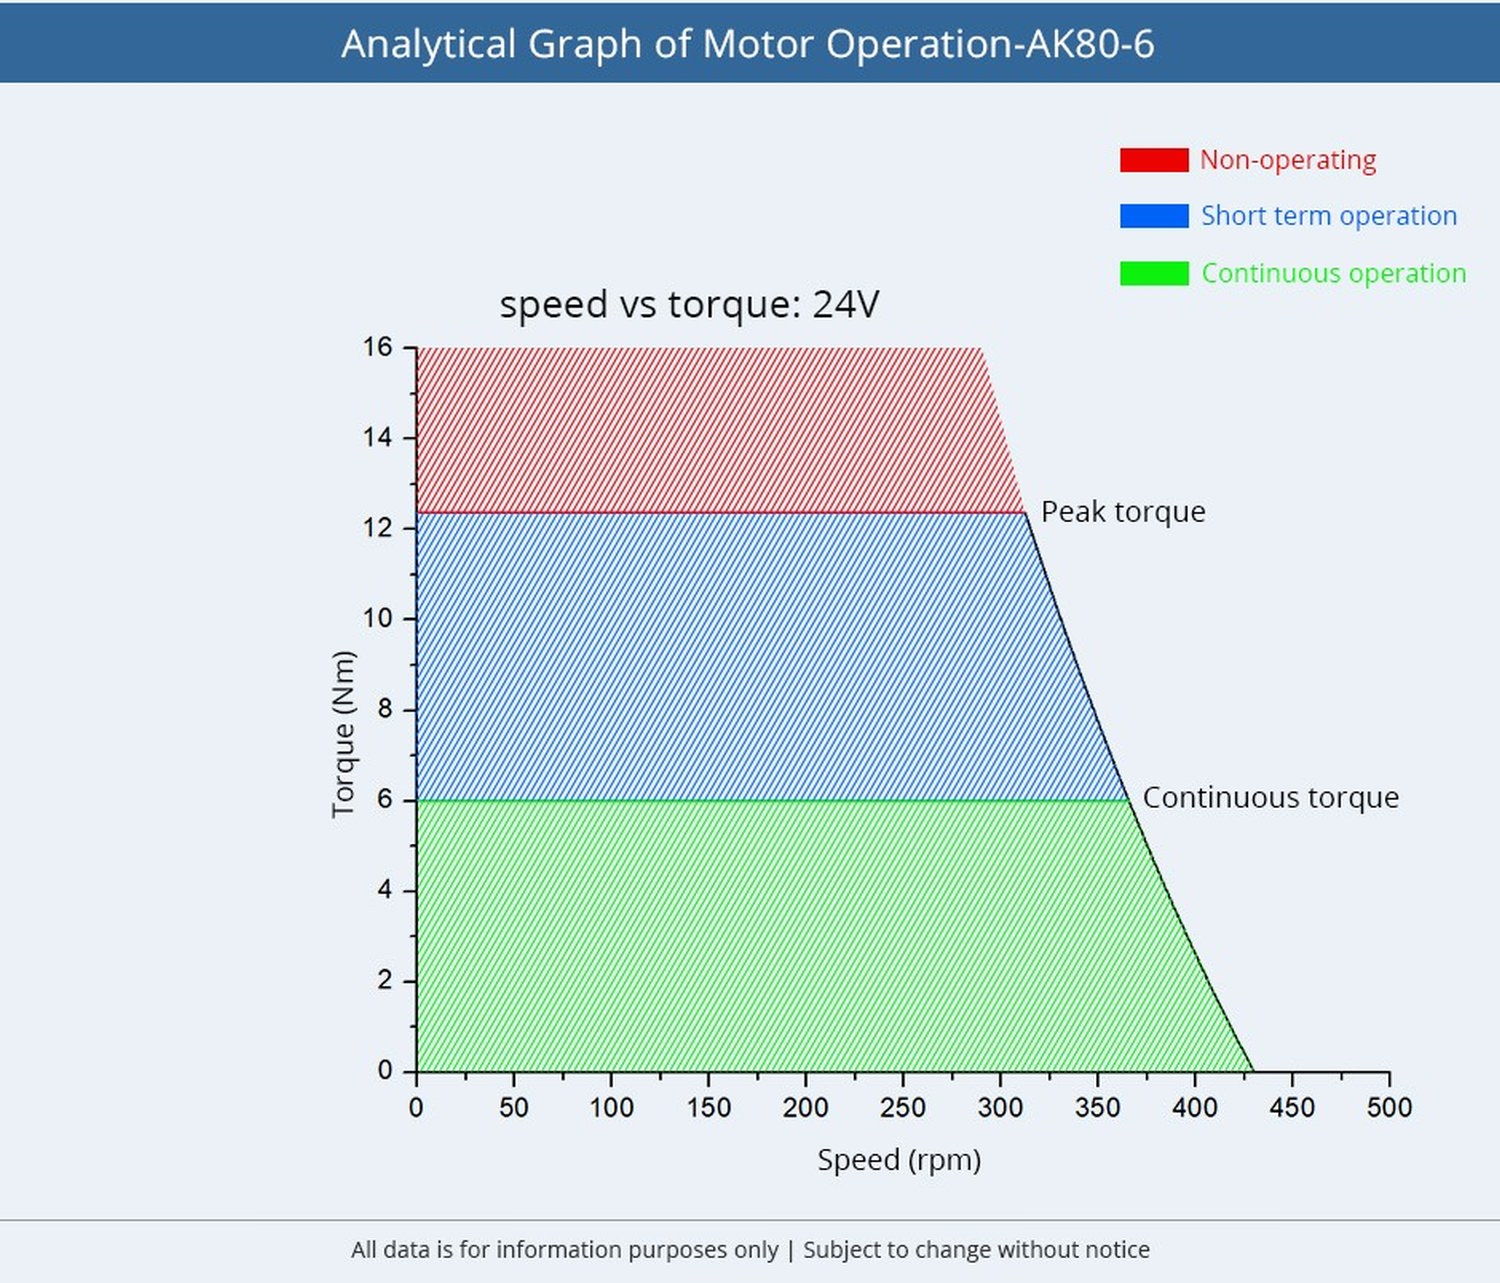
\includegraphics[width=\textwidth]{figures/hardware_setup/torque_speed_curve.jpg}
    \label{fig:subfigb}
    \caption{Speed-torque diagramm}
  \end{subfigure}
  \caption{Quasi direct drive motor}
  \label{fig:twosubfigures}
\end{figure}

For communication, We have chosen CAN in this implementation. The Controller Area Network (CAN) bus is a robust, flexible, and efficient communication protocol that has been employed in various applications. There are many advantages to using the CAN bus for control. The CAN bus provides error checking and fault confinement capabilities. It operates in real-time, enabling high control frequencies with relatively simple wiring. In our configuration, there is only one master node (the PC) and two slave nodes (two motors). The control loop simply consists of a CAN-to-USB converter, one CAN high cable, and one CAN low cable, with a termination resistor of \(120 \Omega\) at both ends. The detailed connection is depicted in the figure below:

\begin{figure}[H]
    \centering
    \includegraphics[width=0.7\linewidth]{example-image}
    \caption{CAN connection}
    \label{fig:my_label}
\end{figure}

To ensure a higher control frequency of around 500 Hz, we chose the CAN-USB/2 product from ESD GmbH Hannover. This specialized CAN-to-USB interface utilizes USB 2.0, which supports a data rate of 480 Mbit/s. Its CAN capability is 1 Mbit/s, in accordance with ISO 11898-2. Additionally, it supports the SocketCAN interface included in the Linux Kernel 2.6, making it easier to use in a Linux development environment.

\begin{figure}[H]
    \centering
    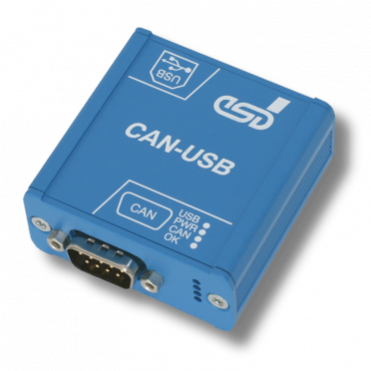
\includegraphics[width=0.3\linewidth]{figures/hardware_setup/can_blue_box.png}
    \caption{blue box}
    \label{fig:my_label}
\end{figure}

Due to accidents that occurred during testing with the mechanical systems from the first iteration, several safety protocols have been implemented to ensure the safety of both human lives and equipment. Four major measures have been taken.

An emergency stop is connected directly to the 24V power source. If the behavior of the double pendulum deviates from the expected range during testing, the power supply can be manually cut off immediately. The energy in the mechanical system will dissipate rapidly, and the system will return to its initial state automatically.

In scenarios where the system is moving at a very high speed when the emergency stop is engaged, the motors attached to the revolute joints act as generators, dissipating the mechanical energy from the system's motion. The generated current is fed back into the circuit, and in extreme cases, it could overload the power supply. To counteract this, a capacitor is connected to the power supply to absorb any electrical surge resulting from a sudden stop.

Further, speed and position limits have been set at the software level. As the links of the pendulum can experience vibrations and rotational imbalances at high speeds, potentially leading to structural disassembly, a speed limit of 20 rad/s has been established. Any speed exceeding this value will trigger a full system stop, equivalent to pressing the emergency stop button. The position limit is set to \(2\pi\) for both pos1 and pos2. Excessive rotations could cause the CAN and power cables to become entangled, leading to interference and potential cable damage.

Lastly, to guard against unpredictable system failures, a custom protective cage has been constructed using aluminum profiles and thick acrylic boards. This cage fully encloses the double pendulum hardware, significantly reducing the risk of accidents.

These measures have been instrumental in minimizing potential hazards during testing and operation.

\section{System identification}
System identification is the process of deriving mathematical models of dynamic systems from observed input-output data. This method is fundamental in control theory, used to analyze, predict, and control the behavior of real-world systems. After setting up the hardware system and before transitioning the working model from a successful simulation to the real system, it's necessary to undergo a system identification process. This helps ascertain the real-world parameters governing the dynamics of the double pendulum.

Out of all model parameters, 15 are selected. While the naturally provided parameters \(g\) and \(g_r\) are held constant, the easily measurable parameters \(l_1\) and \(l_2\) are considered independent. The remaining system parameters, which are 
\[
m_1 r_1,\, m_2 r_2,\, m_1,\, m_2,\, I_1,\, I_2,\, I_r,\, b_1,\, b_2,\, c_{f1},\,c_{f2}
\]

need to be identified. The ultimate objective is to discern the parameters of the dynamic matrices present in the equations of motion.
\begin{equation}
M \ddot{q} + C(q, \dot{q}) \dot{q} - G(q) + F(\dot{q}) - D u = 0
\end{equation}

By running excitation trajectories on the actual hardware, data tuples in the form \((q, \dot{q}, \ddot{q}, u)\) can be collected. To determine the most accurate system parameters, one can leverage the linearity of the dynamic matrices \(M\), \(C\), \(G\), and \(F\) in relation to the independent model parameters. Consequently, a least squares optimization can be performed on the recorded data, relative to the dynamics equation.

The identified model parameters are shown in table below:


\section{Sim2Real problem}
Transferring working models from simulation to real systems to produce similar performance has always been a challenge in controller design. This challenge is even more pronounced in model-free reinforcement learning for several reasons.

Firstly, model-free reinforcement learning relies solely on interaction with the environment to gain experience and select actions. While a simulation environment is merely a simplification of the real-world scenario, the agent in simulation might not capture all the factors, such as friction, sensor noise, or real-world dynamics, accurately. Therefore, a control policy optimized for a simplified model might not perform as expected in the more intricate real world.

Secondly, many simulations operate in discrete time and space, whereas the real world functions continuously. In our implementation, the control frequency presents a significant challenge. We use a control frequency of 100 Hz in simulation; however, it does not suffice in the real system. To enhance performance, we increased the control frequency to 400 Hz when experimenting on the real system, and this adjustment yielded positive results.

Thirdly, uncertainties in the environment can lead to substantial complications when attempting to apply learned strategies or actions. Generally speaking, the uncertainty of the environment is addressed by the robustness of the model. However, for highly chaotic systems like the pendubot or acrobot, even slight measurement errors can result in significant deviations from the planned behavior. Our model for controlling the pendubot and acrobot requires a higher level of robustness or a more effective sim2real transfer method.

\subsection{Validation with noisy simulation}

\begin{figure}[htbp]
    \centering
    \fbox{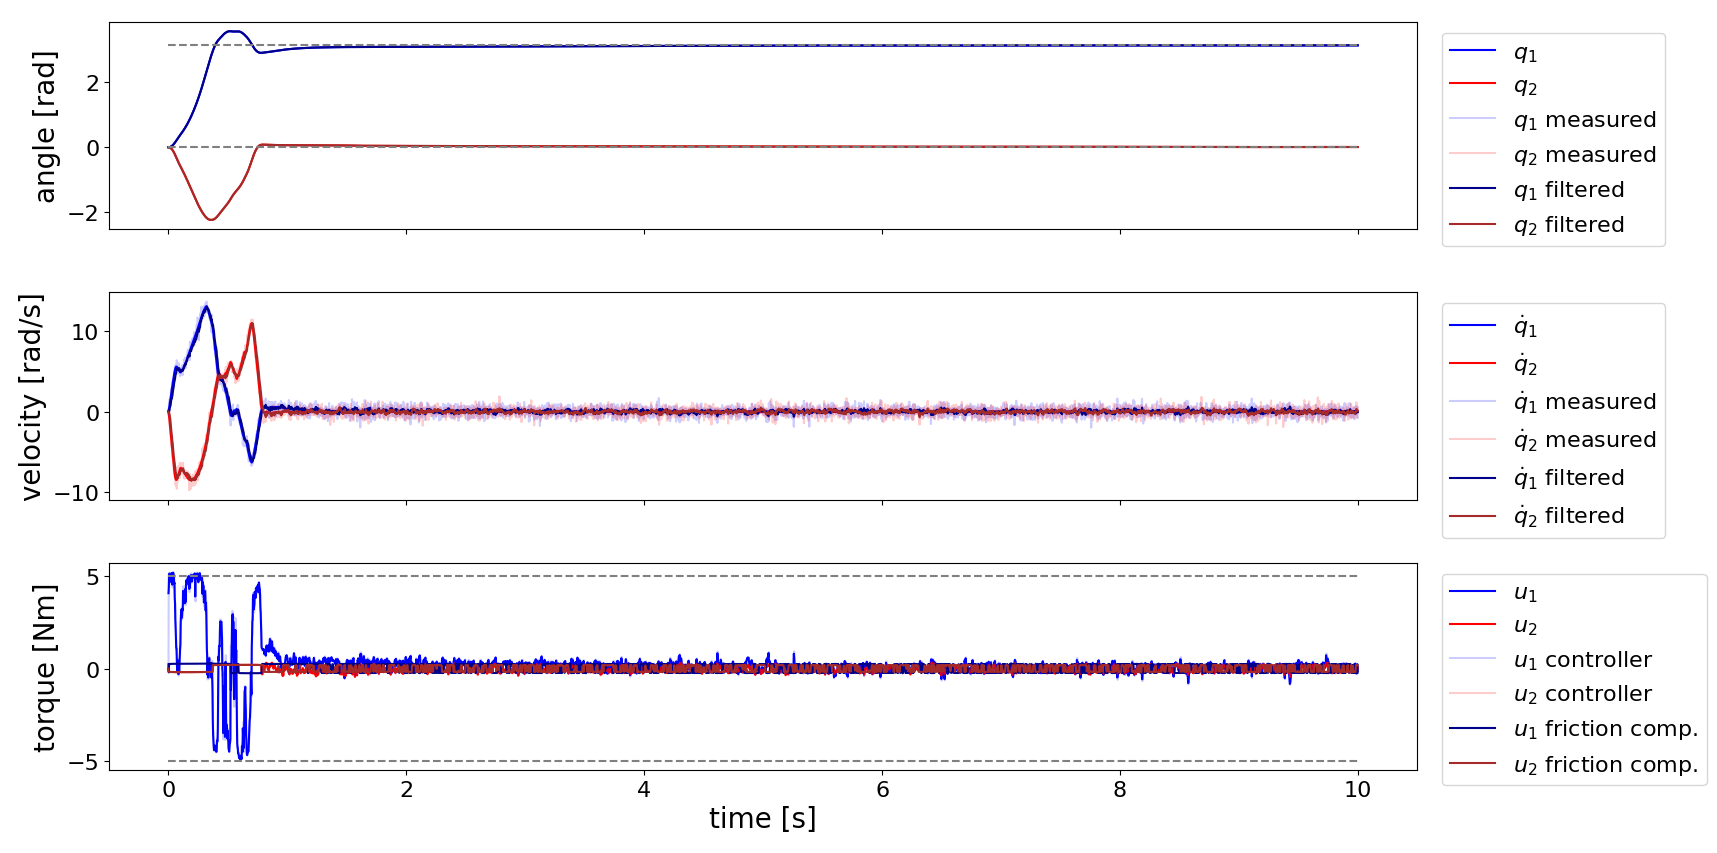
\includegraphics[width=0.9\textwidth]{figures/hardware_result/pendubot_noisy_unclipped.png}} % Second image
    \caption{pendubot noisy simulation result}
    \label{fig:image_b}
\end{figure}
\subsection{Training with domain randomization}



\section{Real hardware results}
This section is about simulation results in pendubot and acrobot.

\subsection{pendubot results}
pendubot:

\begin{figure}[H]
    \centering
    \includegraphics[width=0.7\linewidth]{example-image}
    \caption{Pendubot results on real systems}
    \label{fig:my_label}
\end{figure}

\subsection{acrobot results}
acrobot:

\cleardoublepage
